%% This is file `elsarticle-template-1-num.tex',
%%
%% Copyright 2009 Elsevier Ltd
%%
%% This file is part of the 'Elsarticle Bundle'.
%% ---------------------------------------------
%%
%% It may be distributed under the conditions of the LaTeX Project Public
%% License, either version 1.2 of this license or (at your option) any
%% later version.  The latest version of this license is in
%%    http://www.latex-project.org/lppl.txt
%% and version 1.2 or later is part of all distributions of LaTeX
%% version 1999/12/01 or later.
%%
%% Template article for Elsevier's document class `elsarticle'
%% with numbered style bibliographic references
%%
%% $Id: elsarticle-template-1-num.tex 149 2009-10-08 05:01:15Z rishi $
%% $URL: http://lenova.river-valley.com/svn/elsbst/trunk/elsarticle-template-1-num.tex $
%%
\documentclass[preprint,12pt]{elsarticle}
\newcommand\tab[1][1cm]{\hspace*{#1}}
%% Use the option review to obtain double line spacing
%% \documentclass[preprint,review,12pt]{elsarticle}

%% Use the options 1p,twocolumn; 3p; 3p,twocolumn; 5p; or 5p,twocolumn
%% for a journal layout:
%% \documentclass[final,1p,times]{elsarticle}
%% \documentclass[final,1p,times,twocolumn]{elsarticle}
%% \documentclass[final,3p,times]{elsarticle}
%% \documentclass[final,3p,times,twocolumn]{elsarticle}
%% \documentclass[final,5p,times]{elsarticle}
%% \documentclass[final,5p,times,twocolumn]{elsarticle}

%% The graphicx package provides the includegraphics command.
\usepackage{graphicx}
\graphicspath{ {} }
%% The amssymb package provides various useful mathematical symbols
\usepackage{amssymb}
\usepackage{amsmath}
%% The amsthm package provides extended theorem environments
%% \usepackage{amsthm}

%% The lineno packages adds line numbers. Start line numbering with
%% \begin{linenumbers}, end it with \end{linenumbers}. Or switch it on
%% for the whole article with \linenumbers after \end{frontmatter}.
\usepackage{lineno}
\usepackage{algorithmic}
\usepackage{algorithm2e}

%% natbib.sty is loaded by default. However, natbib options can be
%% provided with \biboptions{...} command. Following options are
%% valid:

%%   round  -  round parentheses are used (default)
%%   square -  square brackets are used   [option]
%%   curly  -  curly braces are used      {option}
%%   angle  -  angle brackets are used    <option>
%%   semicolon  -  multiple citations separated by semi-colon
%%   colon  - same as semicolon, an earlier confusion
%%   comma  -  separated by comma
%%   numbers-  selects numerical citations
%%   super  -  numerical citations as superscripts
%%   sort   -  sorts multiple citations according to order in ref. list
%%   sort&compress   -  like sort, but also compresses numerical citations
%%   compress - compresses without sorting
%%
%% \biboptions{comma,round}

% \biboptions{}

\journal{Journal Name}

\begin{document}

\begin{frontmatter}

%% Title, authors and addresses

\title{Estimation of Phylogenetic Tree using Gene Sequencing Data}

%% use the tnoteref command within \title for footnotes;
%% use the tnotetext command for the associated footnote;
%% use the fnref command within \author or \address for footnotes;
%% use the fntext command for the associated footnote;
%% use the corref command within \author for corresponding author footnotes;
%% use the cortext command for the associated footnote;
%% use the ead command for the email address,
%% and the form \ead[url] for the home page:
%%
%% \title{Title\tnoteref{label1}}
%% \tnotetext[label1]{}
%% \author{Name\corref{cor1}\fnref{label2}}
%% \ead{email address}
%% \ead[url]{home page}
%% \fntext[label2]{}
%% \cortext[cor1]{}
%% \address{Address\fnref{label3}}
%% \fntext[label3]{}


%% use optional labels to link authors explicitly to addresses:
%% \author[label1,label2]{<author name>}
%% \address[label1]{<address>}
%% \address[label2]{<address>}

\author{S. M. Rafiuddin and Most. Jannatul Ferdous}

\address{Bangladesh University of Engineering and Technology, Dhaka}

\begin{abstract}
%% Text of abstract
Phylogenetic tree is an important way in Bioinformatics to find the evolutionary relationship among the biological species. In this research, a proposed model is described for the estimation of phylogenetic tree. To estimate the phylogenetic tree there are certain necessary steps have to consider. Gene sequences are useful data resource to estimate the relationship among species in molecular level. In this research, the approach is to create a fusion between the existing models for the estimation of phylogenetic tree and a population based meta-heuristics approach i.e. Genetic Algorithm.  NCBI's Entrez databases are used for the acquisition of gene sequencing data. Modular parallel approach is applied to handle this dataset efficiently. This paper illustrates a proposed model to create an independent platform for phylogenetic tree estimation. Existing benchmark approaches for tree population that are used for population based meta-heuristic search technique to find the best possible phylogenetic tree estimation for a given set of gene sequence data.  
\end{abstract}

\begin{keyword}
\textbf{phylogenetic tree estimation; bioinformatics; meta-heuristics; genetic algorithm; gene sequence; ncbi entrez database}
%% keywords here, in the form: keyword \sep keyword

%% MSC codes here, in the form: \MSC code \sep code
%% or \MSC[2008] code \sep code (2000 is the default)

\end{keyword}

\end{frontmatter}

%%
%% Start line numbering here if you want
%%


%% main text
\section{Introduction}
\label{S:1}

Phylogenetic Tree is an approach to represent the evolutionary relationship among the biological species in account of their similarities and dissimilarities on genetic characteristics. Phylogenetic tree growing its importance enormously in the field of Bioinformatics, because there is a large field of genetic diversity and its growing in rapid speed. Evolutionary linage is also estimated from phylogenetic trees. To make an estimation of Phylogenetic Tree, gene sequencing data is an important aspect. To represent multi sequence alignment and to identify signatures of conservation of sequence phylogenetic trees are important. It represents how organisms are related. 


Phylogenetic tree can be rooted or non-rooted. In a rooted phylogenetic tree, a path from the root to a node represents an evolutionary path, i.e. it gives directionality to evolutionary time. On the other hand, a non-rooted tree specifies relationships among taxa but it does not represents directionality information. 


There are usually three types of methods for constructing phylogenetic trees based on explicit model of evolution and character [1]—--
\begin{enumerate}[a)] % (a), (b), (c), ...
	\item Maximum Likelihood Methods
    \item Maximum Parsimony Methods 
    \item Pairwise Distance Methods
\end{enumerate}


There are two types of mutations in gene sequence. In synchronous mutation, amino-acid do not changes and in non-synchronous mutation amino acid changes [1]. Recombination occur when the parts of different DNA strands are merged into a single DNA strand [1]. To estimate a phylogenetic tree of a species and to find the evolution and relationship among genes there can have several procedures [1]. Morphological characters are used before to estimate phylogenetic tree, but in modern days the molecular data is the main interest for the estimation of the phylogenetic tree [2].


This research work is to estimate a phylogenetic tree for a species or genes using its gene sequencing data applying meta-heuristics algorithm. As phylogenetic tree estimation is an NP hard problem and it can be solved in polynomial time, our approach is to create the estimation of phylogenetic tree using meta-heuristics algorithm through the entire search space.
% \subsection{Subsection One}

% \begin{table}[h]
% \centering
% \begin{tabular}{l l l}
% \hline
% \textbf{Treatments} & \textbf{Response 1} & \textbf{Response 2}\\
% \hline
% Treatment 1 & 0.0003262 & 0.562 \\
% Treatment 2 & 0.0015681 & 0.910 \\
% Treatment 3 & 0.0009271 & 0.296 \\
% \hline
% \end{tabular}
% \caption{Table caption}
% \end{table}

% \subsection{Subsection Two}



% \begin{figure}[h]
% \centering
\includegraphics[width=0.4\linewidth]{placeholder}
% \caption{Figure caption}
% \end{figure}



% \begin{equation}
% \label{eq:emc}
% e = mc^2
% \end{equation}

\section{Motivation}
There are few specific reasons behind of this research. Phylogenetic tree is an important way to enrich our understanding how species evolved through the evolution process. It create a true measurement of how the species have to classify and it helps us to choose the parameters of classification procedure. Phylogenetic tree of gene sequences would answer various biological questions involving genetic biodiversity of any species. Phylogenetics is growing as an important sub-part of Bioinformatics field. Also this type of research would also create a great interest in forensic analysis. It could help us to find the origin of pathogens [3].


In a world of limited earth surface there are huge biodiversity. We need to preserve their phylogeny identification. For future biodiversity and beyond, this genetic information need to store in this very structure to predict any biological occurrences ever happened [4].




\section{Problem Formulation}
We have the data of gene sequences and we need to estimate the associated phylogenetics tree using gene sequencing data. The standard Genetic Algorithm is used to estimate the best possible phylogenetic tree. 

\section{Literature Review}
\label{S:2}
Recent advancement of phylogenetics are phylogenetic tree analysis, parsimony, distance measurement, likelihood estimation [5] etc. Liang Liu et al. [6] used gene scale data for the estimation of phylogenetic tree. Various tools for implementing the functionalities of phylogenetics are used here.


Genetic distance is an important aspect for determining the phylogenetics of a particular species. If the ancestral sequence is divide into subsequence then it is possible to show mutate and diverge sequence of the phylogenetic tree [1]. 


Neighborhood joining method is another way to achieve phylogenetic identity, in this method, evolution is occurred in every pair in joining and sum of all branches length is measured of that tree [6].


Bayesian phylogenetic analysis is another approach to estimate a position of a species using phylogenetic trees. In this process, interference of phylogeny are determined based on the next stage probabilities of DNA sequence. It creates a conditional probability to calculate the estimation of phylogenetic tree using Bayes theorem [7].


One of the robust methods for the classic changes of phylogenetic analysis is species tree methods using concatenation technique [2]. To find the history of a species of a tree life, genome scale data gives unprecedented opportunities. In comparison with polymerase chain reaction era, some ancient methods like evolutionary genomics and molecular ecology are replaced by new invented methods. 


In recent years, a new method introduced by Hey Nielson, and others, which has been widely used. Bayesian formats has been updated to accommodate whole genome data [8][9][10]. 
Generally two models are used in phylogenetic tree. They are coalescent and concatenation models. Coalescent model is now used over concatenation method for using free recombination among genes [2].


One of the simplest coalescent model that has recently used is multispecies coalescent model (MSC). It builds on the neutral coalescent model for single species, such as Wright- Fisher model [11]. In this model each branch of species is treated as single, neutral coalescent population, and going backwards in time [12].



\section{Proposed Model for Phylogenetic Tree Estimation}

\label{S:3}
As the problem definition is an NP hard problem, there is a huge search space to deal with. Our approach is to use Genetic Algorithm (GA) for this solution procedure. The methodologies will use NCBI's Entrez databases for Gene Sequencing database [13]. The solution procedure are as follows—--


\begin{enumerate}[a)] % (a), (b), (c), ...
	\item Take Gene Sequencing data as initial population.
    \item Retrieve the homologous sequence from the gene sequence data. 



Homologous gene sequence alignment is retrieved by log odds matrices [1], which is defined by—-

$$S(i,j)=S(j,i)=log \frac{q_i*_j}{p_i*p_j}$$
Here, $q_{ij}$ = Probability of finding gene i and gene j aligned in gene sequence.

$p_i$  = Proportion of gene i in sequence and it is the probability of finding i in random position of a gene sequence.

$p_i*p_j$ = Probability of finding gene i and gene j aligned in random.

	\item Find the multiple sequence alignment from the homologous sequence.
\begin{center}
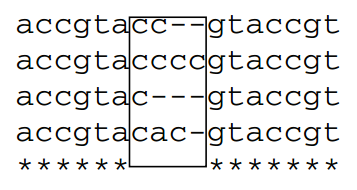
\includegraphics{FIG01.PNG}

\textbf{Fig. 1.} Multiple gene sequence alignment from homologous gene sequencing data.
\end{center}

	Dynamic Programming (DP) is used to find the best alignment with associated scores. If two gene sequence X and Y are aligned in a 2D grid, i is the index of sequence X and j is the index of sequence Y then the best sub-path will be determined by DP as [1]—--
    $$F(i,j)=max\{{F(i-1,j-1)+s(X_i,Y_i),	F(i-1,j)-g,	F(i,j-1)-g}\}$$

	Here, $s(X_i,Y_i)$ is the score defined as substitution matrix in homologous gene sequence. As this formula works for only two sequences, this approach can be generalized for multiple sequence alignment for multiple sequences for more than two sequences. This multiple generalized approach would find the alignment that gives best score for the following formula—--
    $$\sum_{i}^{} W_{ij}D_{ij}$$
    
    Here, $W_{ij}$ is the weight matrix and $D_{ij}$ is the distance matrix of ij grid of multiple sequence alignment.
    
But if gaps of arbitrary size are possible to place in any particular position, then the affine gap penalties formula is used. By this techniques penalties are subtracted from the particular alignment score. Gap Penalties are determined by [1]—--
$$GP=g+e(l-1)$$

Here, $l$ = Length of the gap.

$g$ = gap opening penalty, i.e. charged one for a gap.

$e$ = gap extension penalty, i.e. charged once per start and end of the gap. 
	\item Use the existing model for selecting the initial population. The existing models are as follows--— 
  
\begin{enumerate}[(A)]
\item \textbf{Maximum Likelihood Method}

It is a probability based approach using likelihood function. If the probability of n tosses end with h head and the probability of the toss is $\theta \in [0, 1]$, then the likelihood function is defined as [1]—--
$$L(\theta)=Pr⁡[H=h]= \binom{n}{h} {\theta}^h (1-\theta)^{(n-h)}$$
Maximizing the likelihood function $L(\theta)$ we can get—--
$$L'(\theta)=\frac{\partial log[L(\theta)]}{\partial \theta}=\frac{h}{\theta}=\frac{n-h}{1-\theta}$$
From the above theory, Maximum Likelihood Estimation (MLE) can be achieved for phylogenetic tree as—--
$$L(\tau,\theta)=Pr(Data|\tau,\theta)$$
$$L(\tau,\theta)=Pr(Aligned Gene Sequences| Tree, Model of Evalution)$$
$\tau'$ and $\theta'$ are making the likelihood function maximized---
$$\tau',\theta'=argmax (L(\tau,\theta))$$
\item \textbf{Maximum Parsimony Method}

This approach is for finding the optimal tree have two aspects [1]—--
\begin{enumerate}[(i)]
\item To determine the change of character and tree length.
\item To search the entire space for all possible tree topologies to minimize the tree length.
If $\tau$ is the phylogenetic tree and $N$ is the number of character $l_j$ is the length of a single sequence then the determined length is [1]—--
$$L(\tau)=\sum_{j=1}^{N} l_j$$
If the nodes are terminal, the length of the binary phylogenetic tree is [1]—--
$$l_j=\sum_{k=1}^{2N-3} C_{a(k),b(k)}$$
Here, $a(k)$ and $b(k)$ are states of the node of the branch $k$.
\end{enumerate}


\item \textbf{Pairwise Distance Method}

Pairwise distance method are non-character based and it is an explicit model of evolution. It has two steps [14]—--
\begin{enumerate}[(i)]
\item Evolutionary distances estimation. If $P$ is the percent difference two gene sequence $X$ and $Y$, then we get the genetic distance, $D$ as—--
$$D=- \frac{3}{4} \ln(1-\frac{4}{3}P)$$
\item By the calculated distance, infer the particular tree topology.

From these existing model described above, the phylogenetic tree population are produced, which will be used by the Genetic Algorithms by the following steps—--
\begin{enumerate}[(I)]
\item These initial population that has been chosen from the model will be the input for Genetic algorithm.
\item Estimate the best tree using Genetic Algorithm (GA).

------------------------------------------------------------------------

\textbf{Algorithm 1.} Genetic Algorithm (GA) [15]

------------------------------------------------------------------------

1. \textit{popsize} $\gets$ desired population size

2. \textit{P} $\gets$ {\{ \}}

3. \textbf{for} \textit{popsize} times \textbf{do}

4. \tab \textit{P} $\gets$ \textit{P} $\cup$ {\{new random individual from model selection outcome\}}

5. \textit{Best} $\gets$ [ ]

6. \textbf{repeat}

7. \tab \textbf{for} each individuals $P_i$ $\in$ \textit{P} \textbf{do}

8. \tab \tab AssessFitness ($P_i$)

9. \tab \tab \textbf{if} \textit{Best} = [] or Fitness($P_i$) $>$ Fitness ($Best$)

10. \tab \tab \tab Best $\gets$ $P_i$

11. \tab \textit{Q} $\gets$ \{\}

12. \tab \textbf{for} $popsize/2$ times do

13. \tab \tab Parent $P_a$ $\gets$ SelectWithReplacement(\textit{P})

14. \tab \tab Parent $P_b$ $\gets$ SelectWithReplacement(\textit{P})

15. \tab \tab Children $C_a$, $C_b$ $\gets$ Crossover (Copy($P_a$),Copy($P_b$))

16. \tab \tab \textit{Q} $\gets$ \textit{Q} $\cup$ {Mutate($C_a$), Mutate($C_b$)} 

17. \tab \textit{P} $\gets$ \textit{Q}

18. \textbf{until} \textit{Best} is the ideal solution or we have run out of time

19. \textbf{return} \textit{Best}

\begin{center}
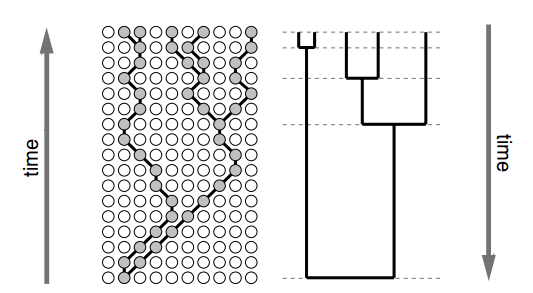
\includegraphics{FIG02.PNG}

\textbf{Fig. 2.} Phylogenetic tree estimation using Genetic Algorithm.
\end{center}
\item Assess fitness from the estimated tree using fitness function.

$$E=\sum_{i=0}^{T-1} \sum_{j=i+1}^{T} W_{ij}|d_{ij}-p_{ij}|^\alpha$$
Here, $E$ = Error of fitting estimates and the tree.

$T$ = Number of taxa.

$d_{ij}$= Distance between taxa $i$ and $j$.

$p_{ij}$= Path length between taxa $i$ and $j$.

$W_{ij}$= Weight to separate the taxa $i$ and $j$.

$\alpha$ = Arbitrary value between 1 and 2.

\item Estimate best tree with measures of support.

\end{enumerate}

\end{enumerate}

\end{enumerate}
\item Test hypothesis result.
\end{enumerate}
\begin{center}
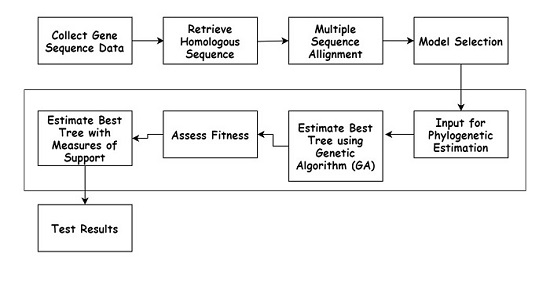
\includegraphics{FIG03.jpg}

\textbf{Fig. 3.} Diagram of the proposed system for the estimation of phylogenetic trees.
\end{center}
\section{Experiments and Results}

	\subsection{Dataset Description}
    The experiment of this research project dataset is NCBI's Entrez databases [13]. This database is a complete collection of information of molecular biology. This database is publicly available and directly downloadable for all kinds of users [1]. There are nine important NCBI dataset accessible via Geneious.

From these nine database Nucleotide, Unigene, Gene, Popset and Taxonomy dataset are important for estimation of phylogenetic tree for a selected species [1]. 


Nucleotide database contains non-redundant DNA sequence [1]. Unigene is a collection of GenBank sequences important for phylogenetic information grouped by gene [1]. Gene database is a collection of information about genetic loci [1]. PopSet is another kind of dataset includes in NCBI's Entrez databases which is important for the estimation of phylogenetic trees because it contains the information of multiple sequence alignments of DNA sequences of different populations of species [1]. Taxonomy contains the information of all species, sub-species and higher and lower taxon and their position order for which there is at least one DNA sequence in databases [1].


NCBI's Entrez database size is huge. Reading the entire dataset at a time is not efficient for a single machine. So, the database should parse before use. For example, only Human genome has a size of 116576 kB. This database can be converted to 6.1 GB file [17].
 


\subsection{Experimental Setup}
    
\textbf{Hardware Setup:} 

Processor:  AMD X4 Phenom II 965 BE 3.4GHz

RAM: 8GB DDR3 1333MHz

HDD: 1TB


\textbf{Software Setup:}

Operating System: Linux Mint XFCE 18.2

Programming Language: Python Programming Language

Version: Python 3.4.1

Used packages: Biopython

\subsection{Statistical Measures}
\begin{center}

\begin{tabular}{ |p{2.8cm}|p{2.8cm}|p{2.8cm}|p{2.8cm}|p{2.8cm}|  }
 \hline
 \multicolumn{5}{|c|}{\textbf{TABLE I. 	RESULT ANALYSIS OF PHYLOGENETIC TREE ESTIMATION}} \\
 \hline
Number of gene sequences per process & Origin of Sequence in Database&Number of tree generated using Maximum Likelihood Methods&Number of tree generated using Maximum Parsimony Methods& Number of tree generated using Pairwise Distance Methods\\
 \hline
 500 & 1 & 34 & 41 & 32\\
 1000 & 501 & 56 & 53 & 45\\
 2000 & 1501 & 59 & 62 & 69\\
 3500 & 1251 & 65 & 71 & 74\\
 5500 & 651 & 78 & 92 & 78\\
 \hline
\end{tabular}
\end{center}
\begin{center}

\begin{tabular}{ |p{4cm}|p{4cm}|p{4cm}|}
 \hline
 \multicolumn{3}{|p{12cm}|}{\textbf{TABLE II. RESULT ANALYSIS OF  ERROR ESTIMATION FOR PHYLOGENETIC TREE}} \\
 \hline
Number of population used for Genetic Algorithm Search Space & Number of Generations for Genetic Algorithm Search Space & Error (\%) after GA estimates best possible phylogenetic trees\\
 \hline
6 & 13 & 6.70\\
9 & 21 & 7.84\\
12 & 45 & 7.93\\
21 & 79 & 9.17\\
31 & 133 & 9.89\\
 \hline
\end{tabular}
\end{center}
The following figure depicts the error estimation in brief in terms of population size---

\begin{center}
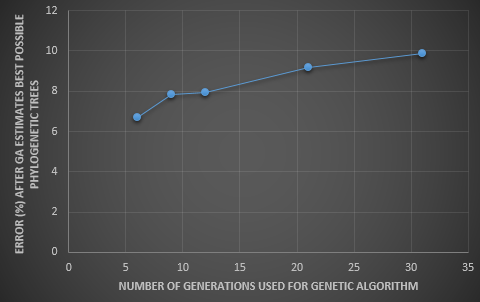
\includegraphics{FIG04.PNG}

\textbf{Fig. 4.} Error (\%) of phylogenetic tree estimation using the fusion of existing model and meta-heuristic approach.
\end{center}

\section{Discussions and Concluding Remarks}
This research has the goal of finding the best possible phylogenetic tree minimizing the error rate. The construction of phylogenetic trees depends on slightly how the gene sequence dataset are organized as well as the model is used for the estimation process. After generating the phylogenetic trees from different models, the trees are applied thorough the Genetic Algorithm using population genetics to find the best possible phylogenetic tree for a particular species. This proposed system for estimating phylogenetic tree shows that using meta-heuristic approaches for a certain search space can come up with better phylogenetic tree with minimum error rate. However, the more gene sequence it gets, the more processing time it needs to estimate the possible phylogenetic tree. So, it needs a higher processing power to deal with a large gene sequence database to estimate phylogenetic tree for a particular species. To know the evolutionary relationship of a species, phylogenetic tree estimation will grow more attention in future research field of bioinformatics. The future work of this research is to optimize the approach up to a certain level to cope up with processing time and minimize the error rate


\section*{Acknowledgement}
The author(s) would like to thank Professor Dr. Mohammad Sohel Rahman, Department of Computer Science and Engineering (CSE), Bangladesh University of Engineering and Technology (BUET) for his kind support and enthusiasm. Also this research work is very much grateful to Pavel Pevzner, Distinguished Professor, Department of Computer Science, University of California, San Diego and Phillip Campeau, Assistant Teaching Professor, Department of Computational Biology, Carnegie Mellon University for their MOOC course on Bioinformatics in Coursera [18]. 
%% The Appendices part is started with the command \appendix;
%% appendix sections are then done as normal sections
%% \appendix

%% \section{}
%% \label{}

%% References
%%
%% Following citation commands can be used in the body text:
%% Usage of \cite is as follows:
%%   \cite{key}          ==>>  [#]
%%   \cite[chap. 2]{key} ==>>  [#, chap. 2]
%%   \citet{key}         ==>>  Author [#]

%% References with bibTeX database:

%% Authors are advised to submit their bibtex database files. They are
%% requested to list a bibtex style file in the manuscript if they do
%% not want to use model1-num-names.bst.

%% References without bibTeX database:

%% Text of abstract
\section*{Reference}
\begin{thebibliography}{1}

\bibitem@
Lemey, Philippe. The phylogenetic handbook: a practical approach to phylogenetic analysis and hypothesis testing. Cambridge University Press, 2009.

\bibitem@
Liu, Liang, et al. "Estimating phylogenetic trees from genome‐scale data." Annals of the New York Academy of Sciences 1360.1 (2015): 36-53.

\bibitem@
Vzquez, Diego P., and John L. Gittleman. "Biodiversity conservation: does phylogeny matter?." Current Biology 8.11 (1998): R379-R381.

\bibitem@
Soltis, Douglas E., and Pamela S. Soltis. "The role of phylogenetics in comparative genetics." Plant Physiology 132.4 (2003): 1790-1800.

\bibitem@
Yang, Ziheng, and Bruce Rannala. "Molecular phylogenetics: principles and practice." Nature Reviews Genetics 13.5 (2012): 303-314.

\bibitem@
Bruno, William J., Nicholas D. Socci, and Aaron L. Halpern. "Weighted neighbor joining: a likelihood-based approach to distance-based phylogeny reconstruction." Molecular biology and evolution 17.1 (2000): 189-197.

\bibitem@
Huelsenbeck, John P., and Fredrik Ronquist. "MRBAYES: Bayesian inference of phylogenetic trees." Bioinformatics 17.8 (2001): 754-755.

\bibitem@
Hey, J. \& R. Nielsen. 2007. Integration within the Felsen-stein equation for improved Markov chain Monte Carlo methods in population genetics. Proc. Natl. Acad. Sci. U.S.A. 104: 2785–2790.

\bibitem@
Machado, C.A. et al. 2002. Inferring the history of spe-ciation from multilocus DNA sequence data: the case of Drosophila pseudoobscura and close relatives. Mol. Biol. Evol. 19: 472–488.

\bibitem@
Wakeley, J. \& J. Hey. 1997. Estimating ancestral population parameters. Genetics 145: 847–855.

\bibitem@
Rannala, B. \& Z. Yang. 2003. Bayes estimation of species divergence times and ancestral population sizes using DNA sequences from multiple loci. Genetics 164: 1645–1656.

\bibitem@
Degnan, J.H. \& N.A. Rosenberg. 2009. Gene tree discordance, phylogenetic inference, and the multispecies coalescent.    Trends Ecol. Evol. 24: 332–340.

\bibitem@
Maglott, Donna, et al. "Entrez Gene: gene-centered information at NCBI." Nucleic acids research 39.suppl 1 (2011): D52-D57.

\bibitem@
Jukes, Thomas H., Charles R. Cantor, and H. N. Munro. "Evolution of protein molecules." Mammalian protein metabolism 3.21 (1969): 132.

\bibitem@
Luke, Sean. Essentials of metaheuristics. Vol. 113. Raleigh: Lulu, 2009.

\bibitem@
Beerli, Peter. "Effect of unsampled populations on the estimation of population sizes and migration rates between sampled populations." Molecular Ecology 13.4 (2004): 827-836.

\bibitem@
Chang, Jeff, et al. "Biopython Tutorial and Cookbook." (2010).

\bibitem@
Bioinformatics MOOC course Specialization in Coursera, "https://www.coursera.org/specializations/bioinformatics"

\end{thebibliography}


\end{document}

%%
%% End of file `elsarticle-template-1-num.tex'.